\documentclass[tikz,border=7pt]{standalone}
\usepackage[T1]{fontenc}
\usepackage{lmodern}
\usepackage{helvet}
\renewcommand{\familydefault}{\sfdefault}
\usepackage{amsmath}
\usepackage{xcolor}
\usepackage{tikz}
\usetikzlibrary{
  arrows.meta,
  positioning,
  calc,
  fit,
  shapes.geometric,
  shapes.symbols,
  backgrounds,
  decorations.pathreplacing,
  decorations.pathmorphing,
}

\definecolor{slate}{HTML}{334155}
\definecolor{teal}{HTML}{0D9488}
\definecolor{amber}{HTML}{D97706}
\definecolor{rose}{HTML}{E11D48}
\definecolor{muted}{HTML}{64748B}
\definecolor{line}{HTML}{94A3B8}
\definecolor{pagebg}{HTML}{F8FAFC}
\definecolor{card}{HTML}{FFFFFF}
\definecolor{lightteal}{HTML}{CCFBF1}
\definecolor{lightamber}{HTML}{FEF3C7}
\definecolor{lightrose}{HTML}{FFE4E6}
\definecolor{lightslate}{HTML}{E2E8F0}
\definecolor{blueink}{HTML}{2563EB}
\definecolor{bluewash}{HTML}{DBEAFE}
\definecolor{greenink}{HTML}{16A34A}
\definecolor{greenwash}{HTML}{DCFCE7}
\definecolor{pinkink}{HTML}{DB2777}
\definecolor{pinkwash}{HTML}{FCE7F3}

\tikzset{
  >=Stealth,
  font=\sffamily\scriptsize,
  every node/.append style={text=slate},
  title/.style={font=\sffamily\bfseries\small, text=slate, anchor=west},
  note/.style={font=\sffamily\tiny, text=muted, align=left},
  label/.style={font=\sffamily\tiny, text=muted},
  chip/.style={
    draw=#1,
    fill=#1!12,
    rounded corners=2pt,
    inner sep=2.5pt,
    font=\sffamily\tiny\bfseries,
    text=slate,
  },
  decision/.style={
    shape=diamond,
    aspect=2.1,
    draw=teal,
    fill=lightteal,
    inner sep=1.5pt,
    align=center,
    font=\sffamily\tiny,
    text=slate,
  },
  pics/person/.style 2 args={
    code={
      \fill[#1] (0,0.92) circle (0.18);
      \fill[#1]
        (-0.26,0.68)
        .. controls (-0.34,0.42) and (-0.30,0.18) .. (-0.22,0.02)
        -- (0.22,0.02)
        .. controls (0.30,0.18) and (0.34,0.42) .. (0.26,0.68)
        -- cycle;
      \node[font=\sffamily\tiny\bfseries, text=#1, anchor=north] at (0,-0.08) {#2};
    }
  },
  pics/disk/.style={
    code={
      \fill[lightslate] (0,-0.04) ellipse (0.28 and 0.10);
      \fill[slate] (-0.28,-0.04) rectangle (0.28,0.12);
      \fill[slate] (0,0.12) ellipse (0.28 and 0.10);
      \fill[card] (0,0.14) ellipse (0.11 and 0.04);
    }
  },
}

\begin{document}
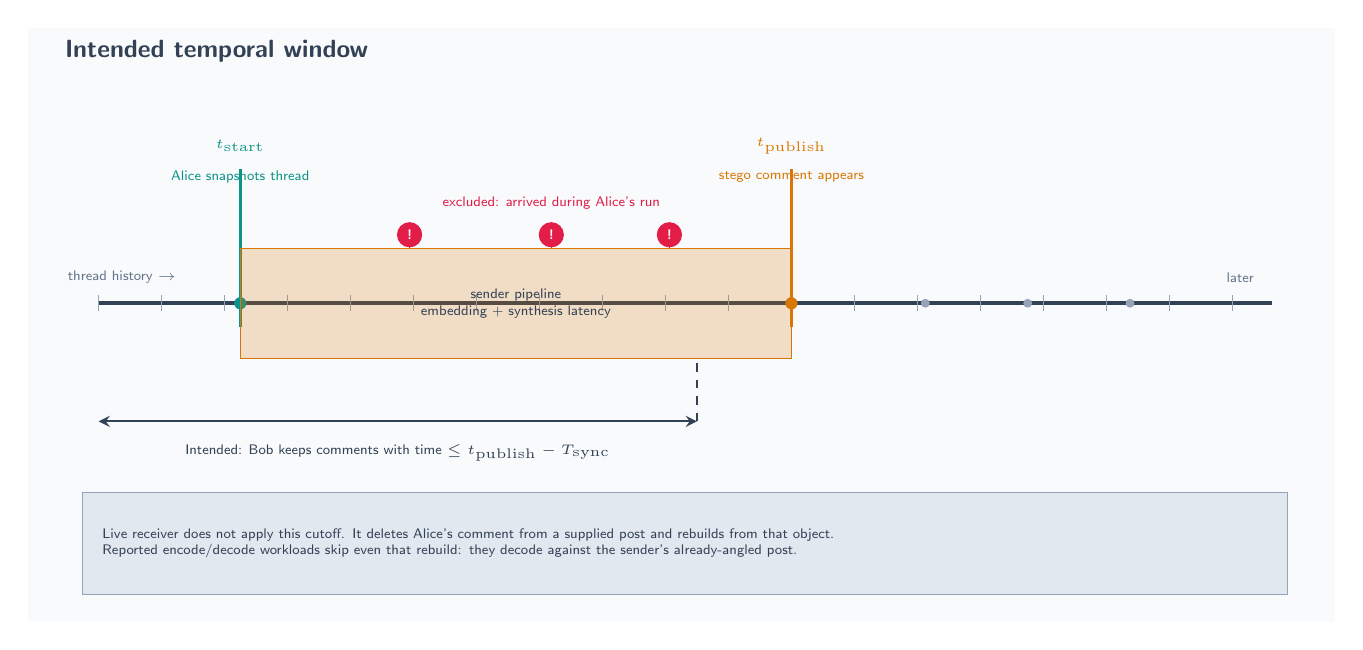
\begin{tikzpicture}[x=1cm,y=1cm]
  \fill[pagebg] (-0.3,-0.2) rectangle (16.3,7.35);
  \node[title] at (0.05,7.05) {Intended temporal window};

  % ruler
  \draw[slate, line width=1.6pt] (0.6,3.85) -- (15.5,3.85);
  \foreach \x in {0.6,1.4,...,15.5} {
    \draw[line] (\x,3.75) -- (\x,3.95);
  }
  \node[label] at (0.9,4.18) {thread history $\rightarrow$};
  \node[label] at (15.1,4.18) {later};

  % t_start
  \draw[teal, line width=1.2pt] (2.4,3.55) -- (2.4,5.55);
  \fill[teal] (2.4,3.85) circle (2.2pt);
  \node[font=\sffamily\tiny\bfseries, text=teal, align=center] at (2.4,5.85) {$t_{\mathrm{start}}$};
  \node[label, text=teal, align=center, text width=3.2cm] at (2.4,5.45) {Alice snapshots thread};

  % latency band
  \fill[amber, opacity=0.22] (2.4,3.15) rectangle (9.4,4.55);
  \draw[amber] (2.4,3.15) rectangle (9.4,4.55);
  \node[font=\sffamily\tiny, align=center] at (5.9,3.85) {sender pipeline\\embedding + synthesis latency};

  % excluded comments as bubbles
  \foreach \x/\lab in {4.55/c$^\ast$, 6.35/c$^\ast$, 7.85/c$^\ast$} {
    \fill[rose] (\x,4.72) circle (0.16);
    \node[font=\sffamily\tiny\bfseries, text=card] at (\x,4.72) {!};
    \draw[rose] (\x,4.56) -- (\x,4.55);
  }
  \node[font=\sffamily\tiny, text=rose] at (6.35,5.12) {excluded: arrived during Alice's run};

  % t_publish
  \draw[amber, line width=1.2pt] (9.4,3.55) -- (9.4,5.55);
  \fill[amber] (9.4,3.85) circle (2.2pt);
  \node[font=\sffamily\tiny\bfseries, text=amber, align=center] at (9.4,5.85) {$t_{\mathrm{publish}}$};
  \node[label, text=amber, align=center, text width=3.4cm] at (9.4,5.45) {stego comment appears};

  % later comments
  \foreach \x in {11.1,12.4,13.7} {
    \fill[line] (\x,3.85) circle (1.6pt);
  }

  % T_sync bracket
  \draw[slate, stealth-stealth, thick] (0.6,2.35) -- (8.2,2.35);
  \draw[slate, dashed] (8.2,2.35) -- (8.2,3.15);
  \node[font=\sffamily\tiny, align=center] at (4.4,1.95) {Intended: Bob keeps comments with time $\leq t_{\mathrm{publish}}-T_{\mathrm{sync}}$};

  % live note
  \fill[lightslate] (0.4,0.15) rectangle (15.7,1.45);
  \draw[line] (0.4,0.15) rectangle (15.7,1.45);
  \node[font=\sffamily\tiny, text width=14.8cm, align=left] at (8.05,0.80) {%
    Live receiver does not apply this cutoff. It deletes Alice's comment from a supplied post and rebuilds from that object.\\
    Reported encode/decode workloads skip even that rebuild: they decode against the sender's already-angled post.};
\end{tikzpicture}
\end{document}
